% Methodologie/Roberta.tex


\subsection{Utilisation de modèle pré-entraîné Roberta}

\subsubsection{Initialisation du Modèle RoBERTa pour l'Analyse de Sentiments}
\begin{figure}[h]
    \centering
    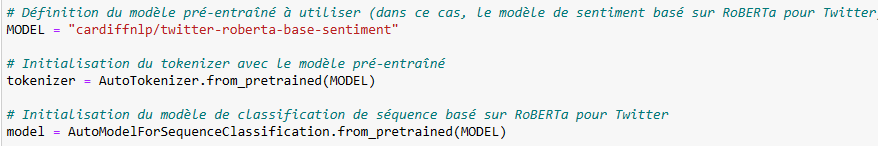
\includegraphics[scale=0.6]{assets/iniRoberta.PNG}
    \caption{initialisation de model RoBERTa}
    \label{fig:initroberta}
\end{figure}
Ces lignes de code définissent le modèle pré-entraîné à utiliser pour l'analyse de sentiments, en l'occurrence le modèle de sentiment basé sur RoBERTa pour Twitter. Le tokenizer associé au modèle est également initialisé, ainsi que le modèle de classification de séquence basé sur RoBERTa pour Twitter. Ces étapes préparent le modèle pour l'analyse ultérieure des sentiments dans le texte.


\subsubsection{Fonction d'Évaluation des Scores de RoBERTa pour l'Analyse de Sentiments}

\begin{figure}[h]
    \centering
    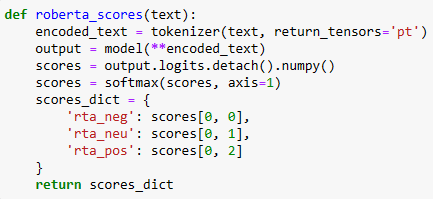
\includegraphics[scale=0.6]{assets/robertaFun.PNG}
    \caption{Fonction d'Évaluation des Scores de RoBERTa}
    \label{fig:evalfunroberta}
\end{figure}
Cette fonction, nommée \texttt{roberta\_scores}, prend en entrée un exemple de texte, l'encode à l'aide du tokenizer associé au modèle RoBERTa pré-entraîné pour l'analyse de sentiments sur Twitter, puis utilise le modèle pour obtenir des scores de sentiment. Les scores sont ensuite normalisés avec la fonction softmax et renvoyés sous forme de dictionnaire comprenant les probabilités associées aux classes négative, neutre et positive.

\subsubsection{Analyse de Sentiments avec RoBERTa sur l'Ensemble de Données}

\begin{figure}[h]
    \centering
    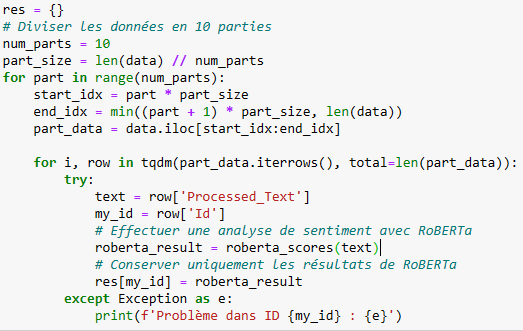
\includegraphics[scale=0.7]{assets/RobertaForAllData.PNG}
    \caption{Applique la fonction sur l'ensemble des donnees}
    \label{fig:applyfunforalldata}
\end{figure}

Ce code parcourt chaque ligne de l'ensemble de données \texttt{data}, récupère le texte et l'identifiant associé, puis utilise la fonction \texttt{roberta\_scores} pour effectuer une analyse de sentiment avec le modèle RoBERTa pré-entraîné. Les résultats de RoBERTa sont ensuite stockés dans un dictionnaire \texttt{res}, associant chaque identifiant à ses scores de sentiment correspondants. En cas d'erreur de type \texttt{RuntimeError}, un message est affiché indiquant l'échec de l'analyse pour un identifiant spécifique.


\subsubsection{Transformation et Fusion des Résultats d'Analyse de Sentiments avec les Données d'Origine}

\begin{figure}[h]
    \centering
    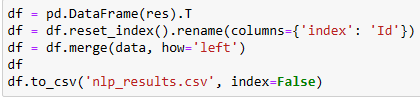
\includegraphics[scale=0.7]{assets/storerobertaresults.PNG}
    \caption{Stocker les resultats du model}
    \label{fig:stockrobertaresults}
\end{figure}

Dans cette phase, les résultats de l'analyse de sentiments avec RoBERTa sont intégrés aux données d'origine. Un DataFrame, \texttt{df}, est créé à partir des scores de sentiment associés à chaque identifiant. Après transposition et réinitialisation, \texttt{df} est fusionné avec l'ensemble de données initial (\texttt{data}) basé sur la colonne 'Id'. Cette fusion permet de combiner les scores de sentiment RoBERTa avec les informations d'origine pour chaque entrée. Le DataFrame final est exporté en CSV sous le nom \texttt{nlp\_results.csv}, facilitant ainsi l'importation ultérieure des résultats pour l'analyse de sentiments.
